\documentclass[a4paper, 12pt]{article}%тип документа

%отступы
\usepackage[left=0.6cm,right=1cm,top=2cm,bottom=3cm,bindingoffset=0cm]{geometry}
\setlength{\parindent}{5ex}

%Русский язык
\usepackage[T2A]{fontenc} %кодировка
\usepackage[utf8]{inputenc} %кодировка исходного кода
\usepackage[english,russian]{babel} %локализация и переносы

%Вставка картинок
\usepackage{graphicx}
\graphicspath{{pictures/}}
\DeclareGraphicsExtensions{.pdf,.png,.jpg}

%Графики
\usepackage{pgfplots}
\pgfplotsset{compat=1.9}

%Математика
\usepackage{amsmath, amsfonts, amssymb, amsthm, mathtools}

%Таблицы
\usepackage{longtable} 
\usepackage{float}

%Римские цифры
\newcommand{\RomanNumeralCaps}[1]{\uppercase\expandafter{\romannumeral#1}}

\usepackage{multirow}


\begin{document}
	\begin{titlepage}
		\begin{center}
			\textsc{Федеральное государственное автономное образовательное учреждение высшего образования«Московский физико-технический институт (национальный исследовательский университет)»\\[5mm]
			}
			
			\vfill
			
			\textbf{Отчёт по лабораторной работы 4.4.1 (5.1)\\[3mm]
				ИЗУЧЕНИЕ ЦЕНТРИРОВАННЫХ
				ОПТИЧЕСКИХ СИСТЕМ
				\\[50mm]
			}
			
		\end{center}
		
		\hfill
		\begin{minipage}{.5\textwidth}
			Выполнил студент:\\[2mm]
			Сериков Алексей Романович\\[2mm]
			группа: Б03-103\\[5mm]
			
		\end{minipage}
		\vfill
		\begin{center}
			Москва, 2023 г.
		\end{center}
		
	\end{titlepage}
	
	\newpage
	\textbf{Аннотация}\\
	
	
	\textbf{Цель работы: }\\
	
	Определить фокусные расстояния тонких
	собирающих и рассеивающих линз, рассчитать их светосилу и оптическую силу,
	также определить фокусное расстояние и положения главных плоскостей сложной
	оптической системы, состоящей из двух тонких линз.\\
	
	\textbf{В работе используются: }\\
	
	Оптическая скамья с набором рейтеров, положительные
	и отрицательные линзы, экран, осветитель с ирисовой диафрагмой и стрелкой, зрительная труба, кольцевые диафрагмы, линейка.\\
	
	\textbf{Теоретические сведения: } \\
	
	Оптическая система называется положительной или собирающей, если падающие лучи после линзы собираются. Если лучи после линзы расходятся от главной оси, то линза - отрицательная. На рис.1 $F_1$ и $F_2$- фокусы, а $a_1$, $a_2$ расстояния от предмета и от изображения до главных плоскостей $H_1$ и $H_2$ соответственно.    
	
	\begin{figure}[H]
		\begin{center}
			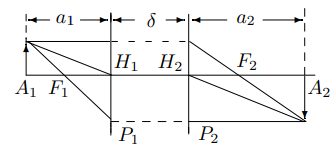
\includegraphics[width = 0.4\textwidth]{1.png}
			\caption{Построение изображения в толстой линзе}
		\end{center}
	\end{figure}
	
	Между $a_1$, $a_2$ и $f$ - фокусным расстоянием системы можно установить соотношение:
	
	\begin{equation}
	\frac{1}{a_1} + \frac{1}{a_2} = \frac{1}{f}.
	\end{equation}
	
	В формуле (1) $a_1$ и $a_2$ берутся со знаком $"+"$, если предмет и изображение реальные, а $f$, если линза положительная.
	Линза считается тонкой, если главные плоскости $P_1$ и $P_2$ почти совпадают и их можно считать в центре линзы.\\
	
	\RomanNumeralCaps 1 \textit{Определение фокусных расстояний тонких линз с помощью экрана:}\\
	
	Чтобы определить фокусные расстояния тонких положительных линз при помощи экрана можно использовать метод Аббе: надо закрепить собирающую линзу между осветителем и экраном. Перемещая осветитель вдоль скамьи, получить на экране резкое изображение
	предмета при двух различных положениях осветителя и
	соответственно экрана (рис. 2)
	
	
	\begin{figure}[H]
		\begin{center}
			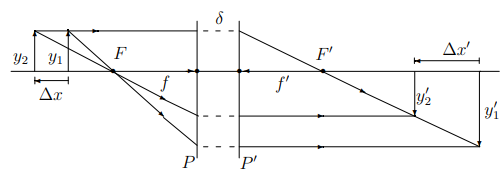
\includegraphics[width = 0.4\textwidth]{2.png}
			\caption{Измерение фокусного расстояния методом Аббе}
		\end{center}
	\end{figure}
	
	Получить фокусное расстояние можно по формуле (2):
	
	\begin{equation}
		f = \frac{\Delta x}{1/\beta_1 - 1/\beta_2} 
	\end{equation}
	Где $\Delta x$ - расстояние между предметами, а $\beta_1 = y_1'/y$ и $\beta_2 = y_2/y$ - линейные увеличения. 
	
	Чтобы определить фокусное расстояние отрицательной линзы сначала с
	помощью одной собирающей линзы нужно получите на экране увеличенное изображение предмета и измерьте расстояние от центра линзы до экрана $a_0$.
	Затем между собирающей линзой и экраном разместить рассеивающую линзу и,
	отодвигая экран от линзы, найти действительное изображение предмета, образованное системой линз. Тогда зная расстояния $a_1$ и $a_2$ (рис. 3), по формуле (1) найдем $f$.
	
	 \begin{figure}[H]
	 	\begin{center}
	 		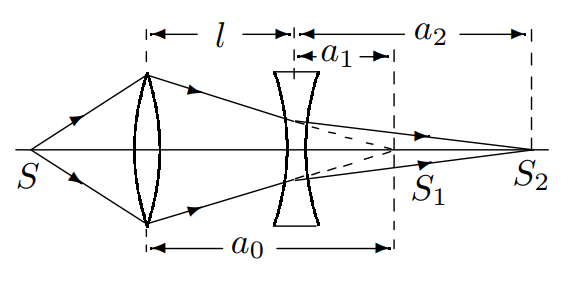
\includegraphics[width = 0.4\textwidth]{3.png}
	 		\caption{Измерение фокусного расстояния отрицательной линзы}
	 	\end{center}
	 \end{figure}
 
 	\RomanNumeralCaps 2 \textit{Определение фокусных расстояний тонких линз с помощью зрительной трубы:}\\
 	
 	Труба должна быть настроена на бесконечность. Если поместив линзу между предметом и трубой, в трубе будет четкое изображение, то предмет находится в фокусе. Для отрицательной линзы нужно использовать схему на рис.3\\
 	
 	\RomanNumeralCaps 3 \textit{Определение фокусного расстояния и положения главных и фокальных плоскостей сложной оптической системы:}\\
 	
 		Для создания сложной оптической системы надо установить близко друг другу две положительные линзы. Для определения фокусного расстояния нужно использовать метод Аббе, и перемещая осветитель, добиться четкого изображения на экране. Поменяв положение предмета, надо получить второй раз четкое изображение. Тогда можно рассчитать фокусное расстояние по формуле (3) и (4):
 		 	\begin{equation}
 		 	f = \frac{\Delta x}{y/y_1' - y/y_2'} = -\frac{\Delta x'}{y_1'/y - y_2'/y}
 		 \end{equation}
 	 \begin{equation}
 	 	-\frac{1}{f} = \frac{1}{f_1} + \frac{1}{f_2} - \frac{|l_12|}{f_1 f_2}.
 	 \end{equation}
  
  	Чтобы найти главные фокусы системы, нужно убрать экран, поставить зрительную трубу, настроенную на бесконечность. После того как получилось четкое изображение в трубе, измерить расстояние $x_1$ от первой линзы со стороны предмета - это положение переднего фокуса, аналогично можно получить значение заднего фокуса системы, если перевернуть линзы.\\
	 
	\textbf{Ход работы и обработка результатов.}\\
	
	\textit{Погрешности измерений:}\\
	Линейка: $\sigma = \pm 2$мм\\
	Формула погрешности произведения и частного:\\
	\begin{equation}
	 \frac{\sigma_u}{u}=\sqrt{\left(\frac{\sigma_x}{x}\right)^2+\left(\frac{\sigma_y}{y}\right)^2}
	\end{equation}
Формула погрешности разности и суммы:
	\begin{equation}
	\sigma_u=\sqrt{\sigma_x^2+\sigma_y^2}
\end{equation}
	 
	 \RomanNumeralCaps 1 \textit{Определение фокусных расстояний тонких линз с помощью экрана:}\\
	 
	 	Сначала производится центрировка элементов оптической системы
	 \begin{enumerate}
	\item Применяем опыт Аббе для положительной линзы, результаты занесем в табл.1 :
	\begin{longtable}{|c|c|c|c|c|c|}
		\hline
		Линза №&$\Delta x$, мм & $\Delta x'$, мм & y, мм & $y_1$, мм & $y_2$, мм \\ \hline
		1 & 111 & 128 & 20 & 62 & 14 \\ \hline
		\caption{Таблица с данными для расчета фокусного расстояния методом Аббе.}
	\end{longtable}
	
	По формуле (2) и (5) подсчитаем величину фокусного расстояния: 
	\underline{$f_1 = 100 \pm 3$ мм} 
	
	\item С помощью положительной линзы определяем фокусного расстояние отрицательной, результаты измерений занесем в табл.2:
	\begin{longtable}{|c|c|c|c|c|}
		\hline
		Линза №&$a_0$, мм & $a_2$, мм & l, мм & a, мм  \\ \hline
		4 & 482 & 113 & 445 & 37 \\ \hline
		\caption{Таблица с данными для расчета фокусного расстояния рассеивающей линзы.}
	\end{longtable}
\end{enumerate}
По формуле (1) и (5) подсчитаем величину фокусного расстояния: 
\underline{$f_4 = 55 \pm 2$ мм} \\

\newpage
\RomanNumeralCaps 2 \textit{Определение фокусных расстояний тонких линз с помощью зрительной трубы:}\\

\begin{enumerate}


\item Исследуем две положительные и одну отрицательную линзы. Для каждой из линз определяем фокусное расстояние с двух сторон ($f_1$ и $f_2$), чтобы понять, можно ли считать данные линзы тонкими.

\begin{longtable}{|c|c|c|}
	\hline
	Линза №&$f_1$, мм & $f_2$, мм \\ \hline
	1 & 92 & 93  \\ \hline
	3 & 110 & 105  \\ \hline
	\caption{Таблица с данными фокусного расстояния положительных линз.}
\end{longtable}
Тогда по формуле (6) получим: \underline{$f_1 = 93 \pm 3$ мм}  и \underline{$f_3 = 108 \pm 3$ мм}\\

\item Для отрицательной линзы используем положительную линзу как на рис.3, где $f = l - a_0$ подученные результаты заносим в табл.4:

\begin{longtable}{|c|c|c|c|}
	\hline
	Линза №&$a_0$, мм & l, мм & $f$, мм  \\ \hline
	4 & 345 & 285 & 60 \\ \hline
	4 & 345 & 280 & 65  \\ \hline
	\caption{Таблица с данными для расчета фокусного расстояния рассеивающей линзы.}
\end{longtable}

Тогда усредним и по формуле (6) получим: \underline{$f_4 = 63 \pm 3$ мм} \\
\end{enumerate}

	\RomanNumeralCaps 3 \textit{Определение фокусного расстояния и положения главных и фокальных плоскостей сложной оптической системы:}\\
	
	\begin{enumerate}
	\item Проведем два измерения для метода Аббе и результаты занесем в табл.5:
	
	\begin{longtable}{|c|c|c|c|c|c|}
		\hline
		Линза №&$\Delta x$, мм & $\Delta x'$, мм & y, мм & $y_1$, мм & $y_2$, мм \\ \hline
		1 и 3 & 47 & 106 & 20 & 50 & 21 \\ \hline
		\caption{Таблица с данными для расчета фокусного расстояния сложной системы.}
	\end{longtable}


По формулам (3), (4) и (5) получим значения фокусного расстояния: \underline{$f = 85 \pm 6$ мм}  и \underline{$f' = 75 \pm 5$ мм}\\

\item Для определения положения главных фокусов поставим зрительную трубу вместо экрана и, когда в ней будет четкое изображение предмета, значит предмет в переднем фокусе системы $F_{1 \Sigma}$. Затем, поменяв линзы местами можем найти положение главного фокуса системы $F_{2 \Sigma}$:

\begin{longtable}{|c|c|c|}
	\hline
	Линза №&$F_{1 \Sigma}$, мм & $F_{2 \Sigma}$, мм  \\ \hline
	1 и 3 & 54 & 57 \\ \hline
	\caption{Таблица с данными главных фокусов сложной системы.}
\end{longtable}
 
\end{enumerate}
	\textbf{Обсуждение результатов и выводы: }\\
	
	Разместим полученные и усредненные результаты в одну таблицу (табл.7):
	
	\begin{longtable}{|c|c|c|c|}
		\hline
		Линза №&$f$, мм &  $\varepsilon _{э}$, \% & $D$, дптр\\ \hline
		1 & 95 & 5&  1\\ \hline
		3 & 108 & 5& 1 \\ \hline
		4 & 59 & 6& 1.7 \\ \hline
		1 и 3 & 80 & 8& 1.25 \\ \hline
		\caption{Таблица с данными фокусных расстояний линз.}
	\end{longtable}
	
	Таким образом можно увидеть, что фокусные расстояния определяются с видимой погрешностью. Основной вклад в ошибку приносит измерение линейкой, так как при некоторых положениях установки проблематично точно провести измерения, так же как и найти центр линзы.

	\end{document}